\section{Elektrische Ladung und elektrisches Feld}
\subsection{Geladene Körper}
\subsubsection{Reibungselektrizität}
Die Reibungselektrizität entsteht durch wiederholten mechanischen Kontakt zwischen 2 unterschiedlichen, nicht leitenden Gegenständen. Dadurch geraten Elektronen vom einen zum anderen Gegenstand.

\subsubsection{Elektrische Ladung im Atom}

Elementarladung $ e \approx 1,6 \ast 10^{-19}C $


\vspace{3mm}
\underline{Ladung:}

\vspace{2mm}
1. Es gibt 2 Arten von Ladung: Positive und Negative. \\
2. Ungleichnamige Ladungen ziehen sich an, gleichnamige Ladungen stoßen sich ab. \\
3. Ein neutraler Körper hat gleich viele positive wie negative Ladungen. \\
4. Positiv geladen = Elektronenmangel. \\
5. Negativ geladen = Elektronenüberschuss. \\
6. In elektrischen Leitern sind Ladungen frei beweglich. \\
7. In der Umgebung von Ladungen existiert ein elektrisches Feld. In ihm wirkt auf andere Ladungen eine Kraft. \\
8. Ein elektrisches Feld kann abgeschirmt werden (mittels eines Faradayschen Käfigs.) \\

\subsubsection{Nachweis elektrischer Ladung}

\vspace{2mm}
\underline{Polarisation:}

\vspace{2mm}
Polarisation ist die Ausrichtung der Dipole in einem Nichtleiter. Dabei richten sich die Dipole so aus, dass die negative Seite zu einer positiven äußeren Ladung zeigt und umgekehrt.

\vspace{2mm}
\underline{Influenz:}

\vspace{2mm}
Influenz ist die Verschiebung der frei beweglichen Elektronen im Metall aufgrund des elektrischen Feldes.

\newpage
\subsection{Messung elektrischer Ladung; Zusammenhang zwischen Ladung und Stromstärke}

\vspace{2mm}
Stromstärke $ I = \dfrac{\Delta Q}{\Delta t} $

\vspace{2mm}
(falls I = const.): $ I = \dfrac{Q}{t} $

\vspace{2mm}
Allgemein: $ I_{(t)} = $ \.{Q}$_{(t)} $ (Stromstärke ist die Ableitung im Q-t-Diagramm)

\vspace{2mm}
[Q] = 1C

\vspace{3mm}
[I] = 1 $ \dfrac{C}{s} $ = 1 A

\vspace{10mm}
\subsection{Die elektrische Kraft zwischen 2 Punktladungen - Das Coulombsche Gesetz}
Die Kraft einer Punktladung Q auf jede Probeladung q, die den Abstand r zur Punktladung hat, kann man mit Hilfe folgender Formel berechnen:

\vspace{3mm}
$ F_{C} = \dfrac{1}{4 \ast \pi \ast \varepsilon _{0} } \ast \dfrac{Q \ast q}{r^{2}} = 9 \ast 10^{9} \dfrac{N \ast m^{2}}{C^{2}} \ast \dfrac{Q \ast q}{r^{2}} $

\vspace{3mm}
Dabei ist $ \varepsilon_{0} \approx 8,85 \ast 10^{-12} \dfrac{C^{2}}{N \ast m^{2}} $

\vspace{3mm}
Die Konstante $ \dfrac{1}{4 \ast \pi \ast \varepsilon _{0} } $ heißt Coulomb-Konstante.

\vspace{5mm}
\underline{Coulombsches Gesetz:}

\vspace{2mm}
Merke:

Die Kraft, die von einer Punktladung auf eine andere ausgeübt wird, wirkt längs der Verbindungslinie zwischen den Ladungen. Sie ändert sich umgekehrt proportional zum quadrat des Abstandes der Ladungen und proportional zum Produkt der Ladungen. \\
Die Kraft ist abstoßend, wenn beide Ladungen gleichnamig sind und anziehend, wenn sie ungleichnamig sind. 

\vspace{3mm}
Vgl. Newtonsches Gravitationsgesetz: $ F_{G} = \gamma \ast \dfrac{M \ast m}{r^{2}} $

\newpage
\subsection{Das elektrische Feld}
Zwei geladene Körper wirken auch über große Distanzen aufeinander ein. Die Wechselwirkung besteht sogar, wenn sich zwischen den Körpern ein Vakuum befindet. Nach dem Feldkonzept herrscht im Raum um einen elektrisch geladenen Körper ein elektrisches Feld $ \vec{E} $, in dem auf andere geladene Körper Kräfte ausgeübt werden. \\
Die elektrische Feldstärke $ \vec{E} $ in einem Punkt des Feldes wird durch 

\vspace{2mm}
$ \vec{E} = \dfrac{\vec{F}}{q} $  \hspace{20mm} [$ \vec{E} $] = 1 $ \dfrac{N}{C} $

\vspace{2mm}
definiert, wobei $ \vec{F} $ die Kraft ist, die auf die Probeladung q wirkt. \\
Das $ \vec{E} $-Feld zeigt in die selbe Richtung wie die Kraft, die auf eine positive Probeladung wirkt. 

\vspace{2mm}
\underline{Elektrische Felder:}
\vspace{2mm}

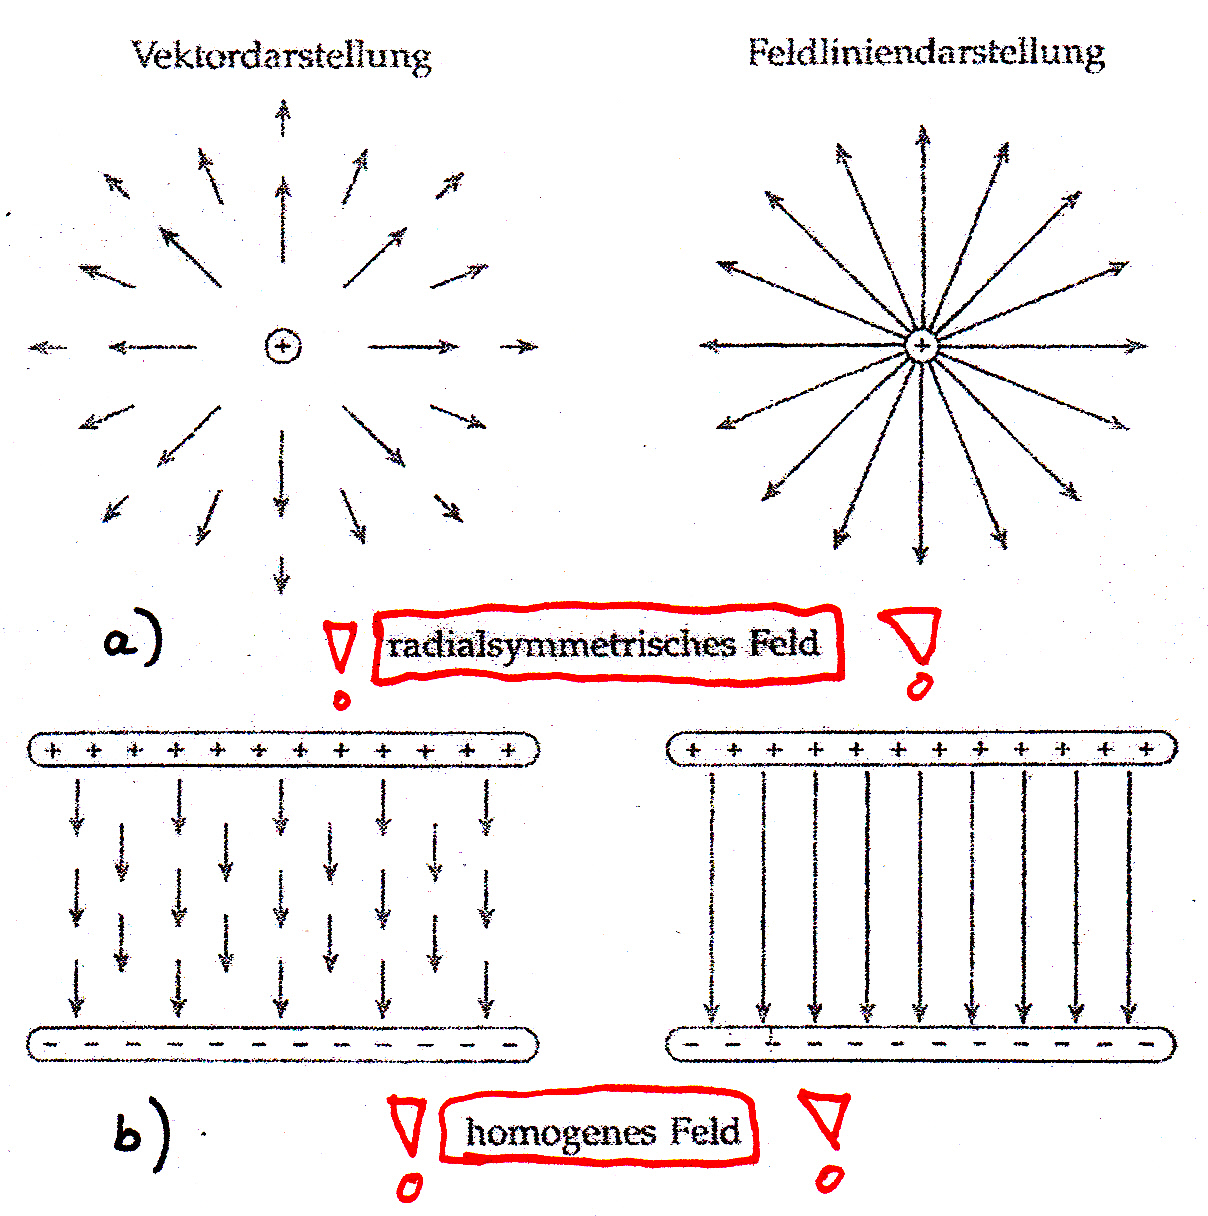
\includegraphics[scale=0.8]{hom_rad_feld}

\vspace{10mm}

\subsection{Darstellung des elektrischen Feldes durch Feldlinien - Aussagen des Feldlinienbildes}
1. An jedem Punkt erfährt eine Probeladung "q" eine Kraft tangential zu den Feldlinien. \\
2. Die Pfeile geben die Richtung der Feldkraft auf eine positive Probeladung an. \\
3. Das Feld ist an Stellen mit größerer Feldliniendichte stärker. \\
4. Feldlinien kreuzen sich nie. \\
5. Die Feldlinien stehen auf einem elektrischen Leiter immer senkrecht.
\vspace{2mm} \\
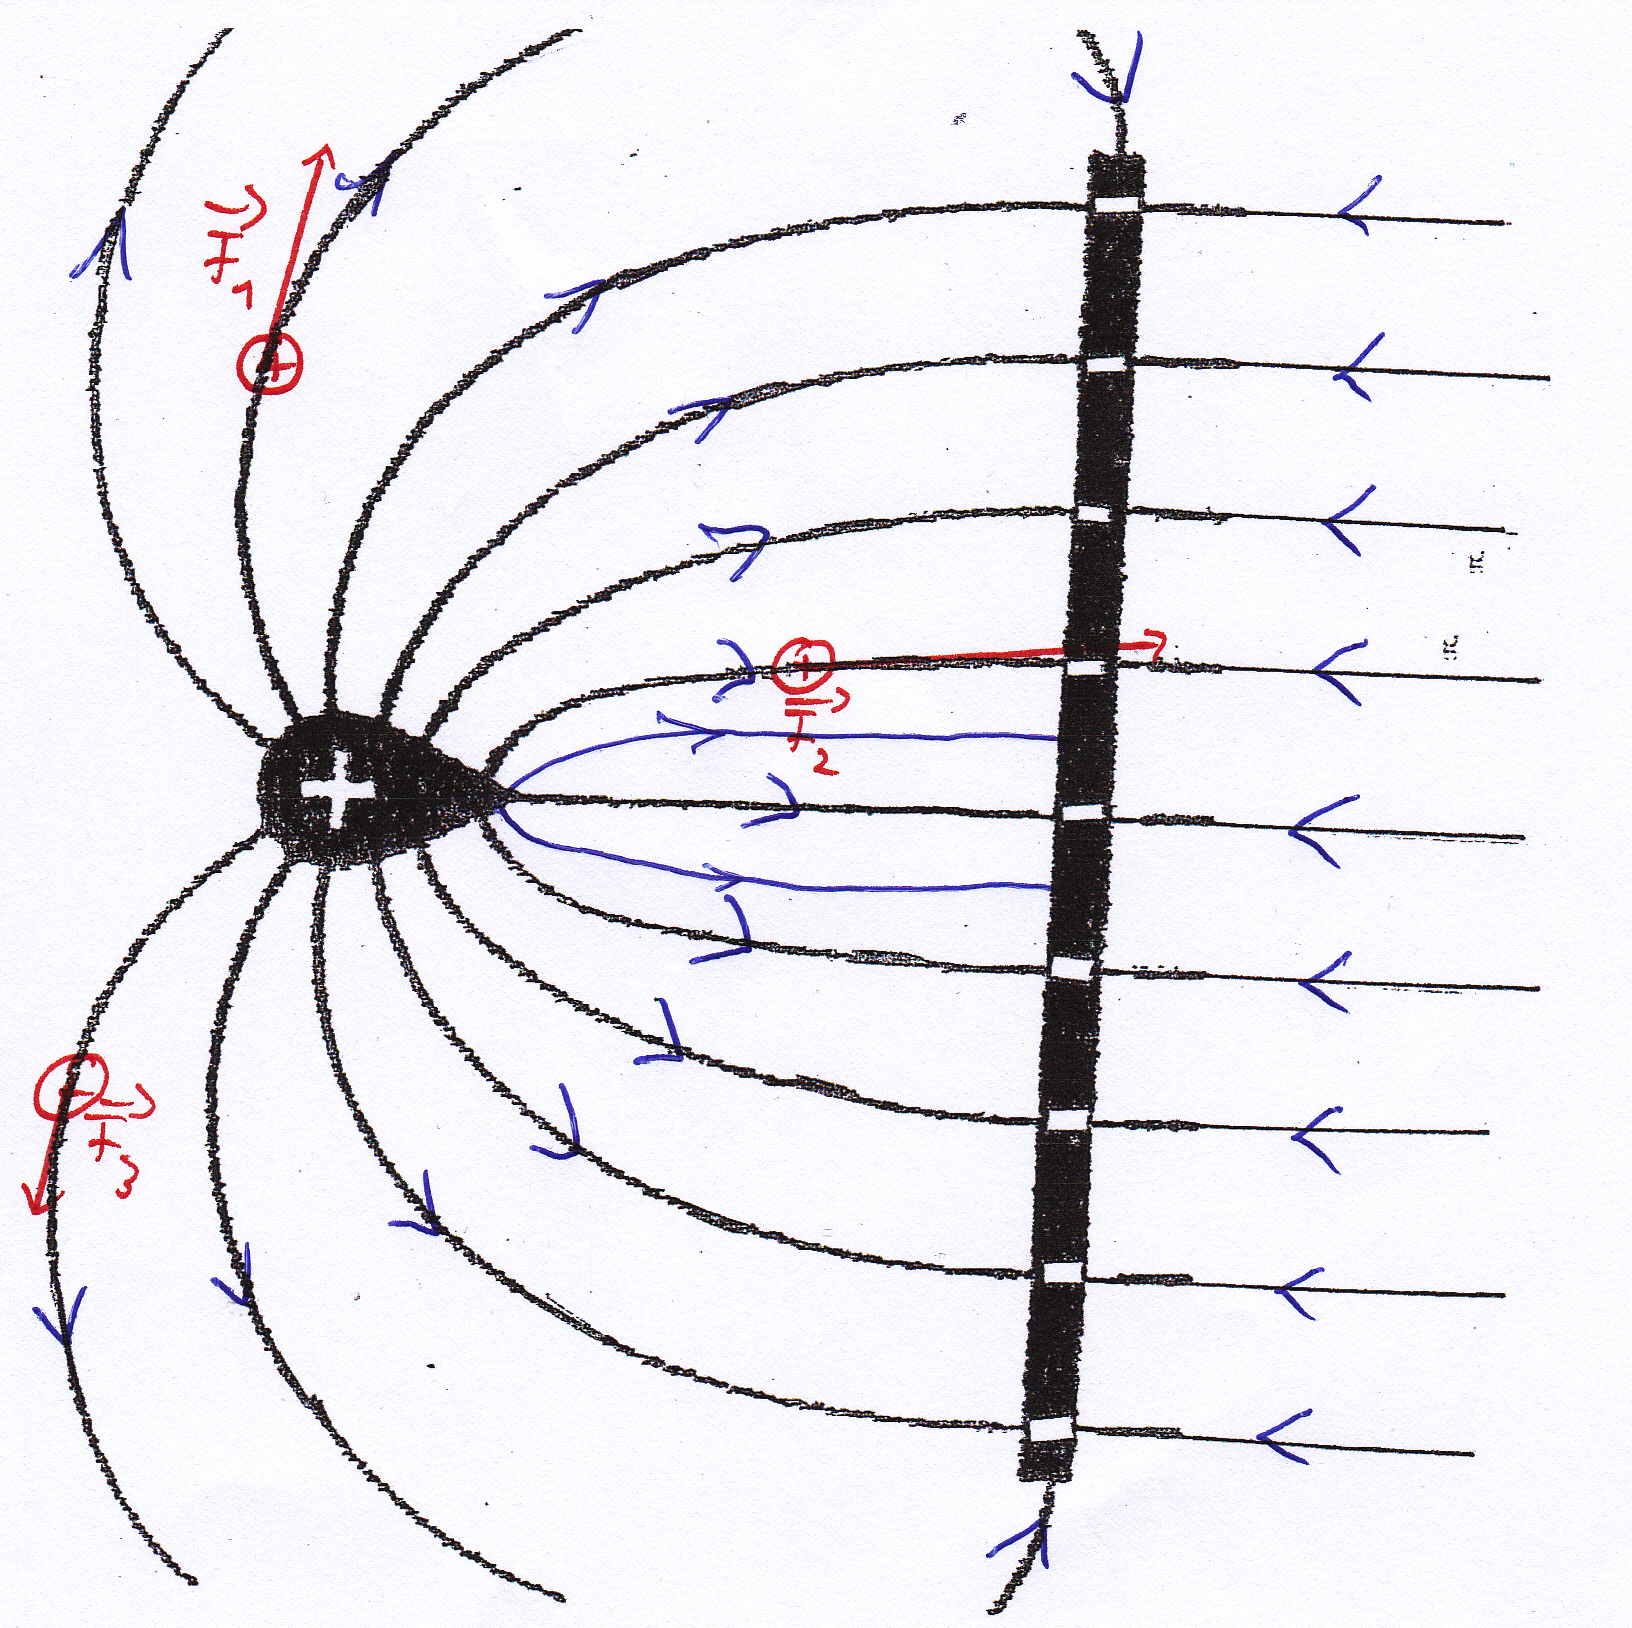
\includegraphics[scale=0.5]{feldlinien_leiter}

\vspace{2mm}
\underline{Merke:}

In der Elektrostatik gilt: \\
1. Feldlinien verlaufen nicht im geschlossenen Kreis, sondern sie beginnen bei positiven Ladungen und enden bei negativen. Wenn eine solche kreisförmige Feldlinie existieren würde, würde sich eine Ladung entlang dieser bewegen und dabei ständig Bewegungsenergie gewinnen ($ \lightning $ Energieerhaltungssatz) \\
2. Feldkräfte können in Leitern Ladungen verschieben. Im Inneren eines Leiters entsteht ein feldfreier Raum. \underline{(Bild faradayscher Käfig)} \\
3. In elektrostatischen Situationen gilt: Das elektrische Feld in einer leitenden Substanz ist überall 0. Die Ladung sitzt auf der Oberfläche der Substanz. \underline{(Bild von Leiter mit Ladung auf Oberfläche)} \\
4. Im Inneren eines Stromführenden Leiters (!Kein elektrostatischer Fall!) besteht ein Feld, das die Ladungen bewegt. 

\vspace{10mm}

\subsection{Vergleich zwischen elektrischem Feld und Gravitationsfeld}
\begin{tabular}{|l|l|l|}
	
	\hline & Gravitationsfeld & Elektrisches Feld\\
	\hline Feld: & Raumbereich, in dem Körper die &   Raumbereich, in dem Ladungen\\
	& Gravitationskräfte $ \vec{F}_{G} $ erfahren.& elektrische Kräfte $ \vec{F}_{el} $ erfahren. \\
	\hline Probekörper: & Probemasse m & Probleladung q \\
	\hline Felderzeugender & Körper mit Masse & Geladene Körper \\
	Körper: & (z.B. Erde) & (Felderzeugende Ladung Q) \\
	\hline Feldlinie: & Gedachte Linie, auf der sich eine & Gedachte Linie, auf der sich eine \\
	& Probemasse bewegt, wenn sie nur & positive Probeladung bewegt, wenn \\
	& der auf sie wirkenden $ F_{G} $ folgt. & sie nur der auf sie wirkenden $ F_{el} $ \\
	& Ihre Tangenten weisen an jeder & folgt. Ihre Tangenten  weisen an \\
	& Stelle der Feldlinie in Richtung & jeder Stelle der Feldlinie in Richtung \\
	& Gravitationskraft $ F_{G} $ & der elektrischen Kraft $ F_{el} $ \\
	\hline Eigenschaften von & 1. Zeigen in Richtung der Kraft & 1. Zeigen in Richtung der Kraft auf \\
	Feldlinien & auf eine Probemasse & eine positive Probeladung \\
	& 2. Zeigen stets zur felderzeugenden & 2. Sie verlaufen von positiver zu \\
	& Masse & negativer Ladung \\
	& 3. Kreuzen sich nie & 3. Kreuzen sich nie \\
	& & 4. Ein elektrischer Dipol stellt sich \\
	& & tangential zur Feldlinie ein. \\
	& & Seine positive Ladung zeigt in \\
	& & Richtung der Feldlinie \\
	\hline Kraft auf: m / q & $ \vec{F}_{G} = m \ast \vec{g} $ & $ \vec{F}_{el} = q \ast \vec{E} $ \\
	\hline Feldstärke & Gravit.-const. $ \vec{g} $ &  Elektr. Feldstärke $ \vec{E} $ \\
	\hline Energie: & $W_{pot} = m \ast g \ast h $ & $ W_{el} = q \ast \vec{E} \ast s = F_{el} \ast s  = q \ast U $ \\
	\hline Potential & $ \varphi_{G} = \dfrac{W_{pot}}{m} = g \ast h $ & $ \varphi_{el} = \dfrac{W_{el}}{q} = E \ast s $ \\
	\hline Potentialdifferenz & $ \varphi_{2} - \varphi_{1} = g \ast \Delta h  $ & $ U = \varphi_{2} - \varphi_{1} = E \ast \Delta s $ \\ \hline
	
\end{tabular}

\subsection{Die Flächenladungsdichte Sigma}
Der Quotient $ \sigma = \dfrac{Q}{A} $ heißt \underline{Flächenladungsdichte}. Die Einheit ist $ [\sigma] = \dfrac{1C}{1 m^{2}} $. \vspace{1mm} Die Feldstärke E eines homogenen Feldes ist der Flächenladungsdichte $ \sigma $ der sie erzeugenden Ladung proportional. \\
In Luft gilt: $ \sigma = \epsilon_{0} \ast \epsilon_{r} \ast E $

\vspace{10mm}

\subsection{Energie, elektrisches Potential und Spannung}
\subsubsection{Energieumwandlung im elektrischen Feld}
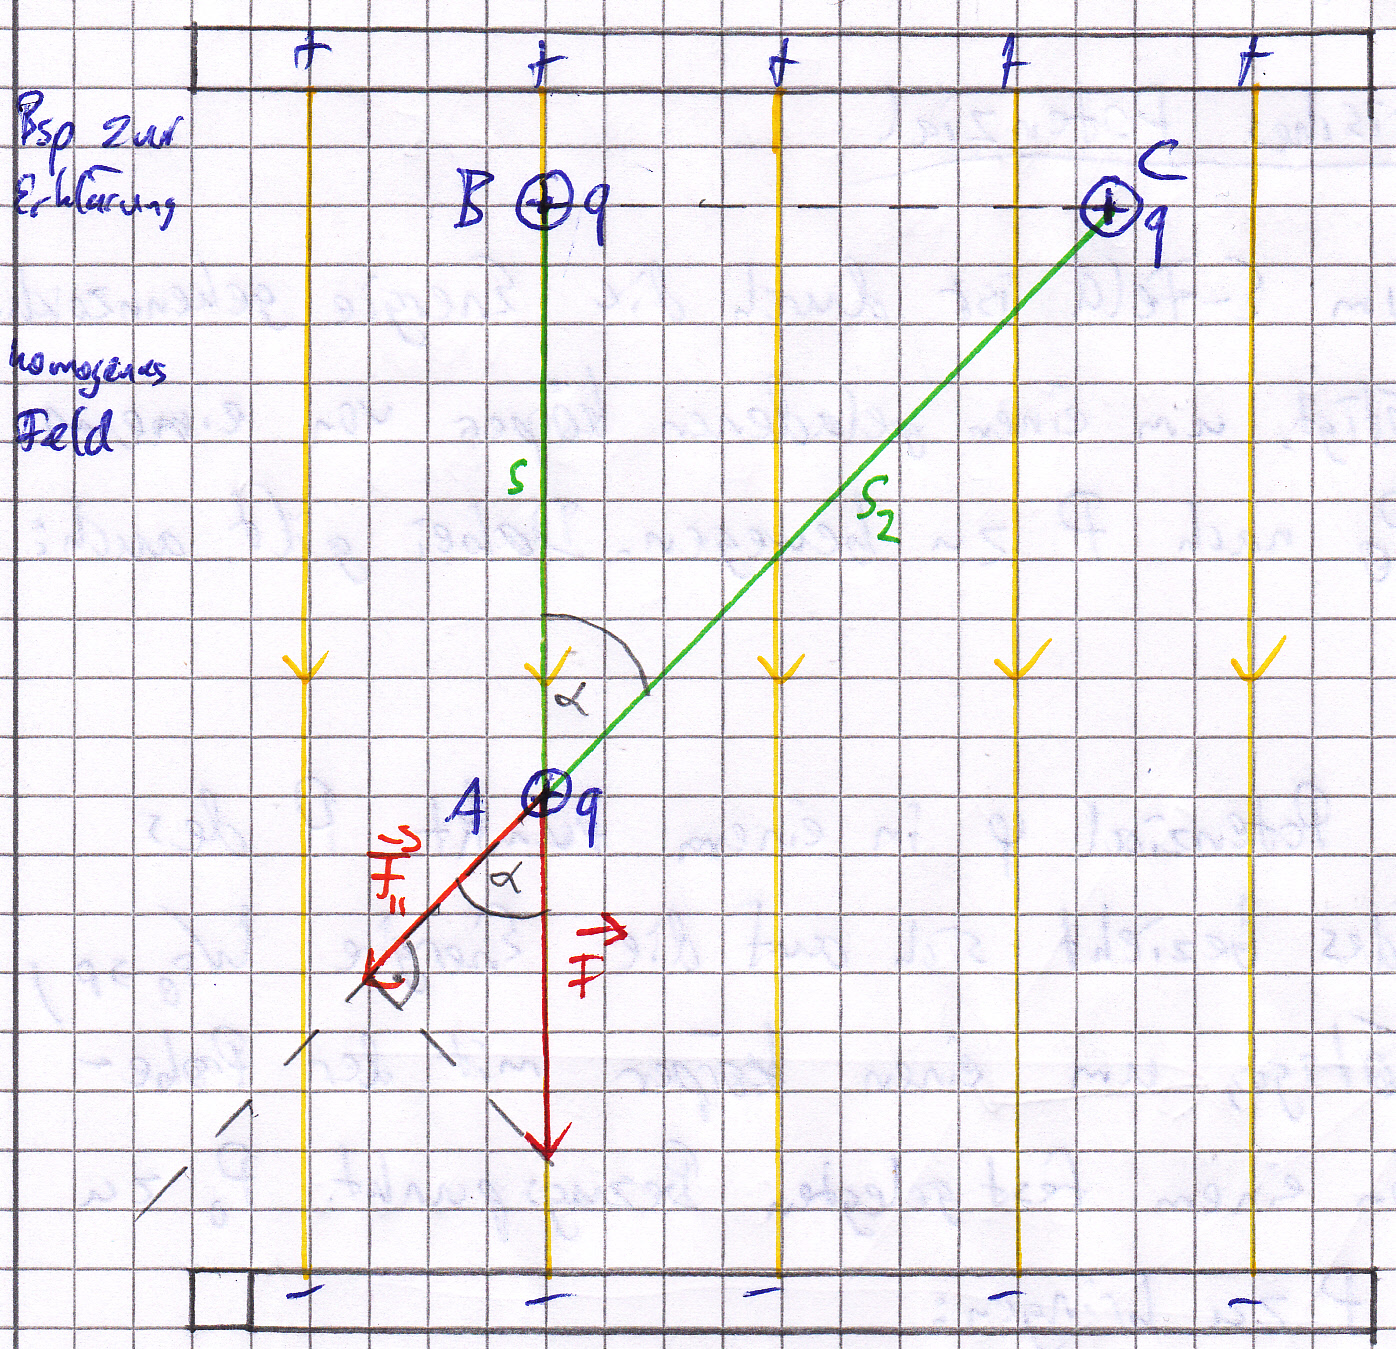
\includegraphics[scale=0.7]{I9_energieumwandlung} \\
Maßstab: 1N $\hat{=}$ 3cm

\vspace{5mm}
$ \vec{F}_{II} = \vec{F} \ast cos(\alpha) $ \hspace{5mm} $ s_{2} = \dfrac{s}{cos(\alpha)} $

\vspace{2mm}
$ W_{A \rightarrow B} = F \ast s $ (In diesem Beispiel: 0,05 J)

\vspace{2mm}
$ W_{A \rightarrow C} = F_{II} \ast s_{2} $ (In diesem Beispiel: 0,05 J)

\vspace{2mm}
$ \Rightarrow W = F \ast s $	

\vspace{2mm}
\underline{Merke:} \\
Verschiebt man einen geladenen Körper im E-Feld entgegen der Kraft, so wird ihm Energie zugeführt. Sie heißt - analog zum Fall des angehobenen Körpers im Gravitationsfeld - \underline{potentielle Energie}. Die Energieänderung bei der Verschiebung einer Ladung ist nur vom \underline{Anfangs- und Endpunkt} abhängig, nicht vom gewählten Weg. Deshalb kann man bei der Berechnung von $W_{pot}$ den Weg in Abschnitte parallel und senkrecht zur Feldlinienrichtung zerlegen, wobei dann nur der parallele Abschnitt einen Beitrag zur Energieänderung liefert. \\
Im \underline{homogenen Feld} ergibt sich: $ W = F \ast s = q \ast E \ast s $ 

\subsubsection{Elektrisches Potential}
Jeder Punkt im E-Feld ist durch die Energie gekennzeichnet, die man benötigt, um einen geladenen Körper von einem Bezugspunkt $P_{0}$ nach P zu bewegen. Dabei gilt auch:
\vspace{2mm} \\
$ W_{P_{0} \rightarrow P} \sim q $
\vspace{2mm} \\
Das elektrische Potential $\varphi$ in einem Punkt P des elektrischen Feldes bezieht sich auf die Energie $W_{P_{0} \rightarrow P}$, die man benötigt, um einen Körper mit der Probeladung q von einem festgelegten Bezugspunkt $P_{0}$ zu diesem Punkt P zu bringen:
\vspace{2mm} \\
$ \varphi_{P} = \dfrac{W_{P_{0} \rightarrow P}}{q} $ \hspace{5mm} $ [\varphi] = \dfrac{J}{C} = V $
\vspace{2mm} \\
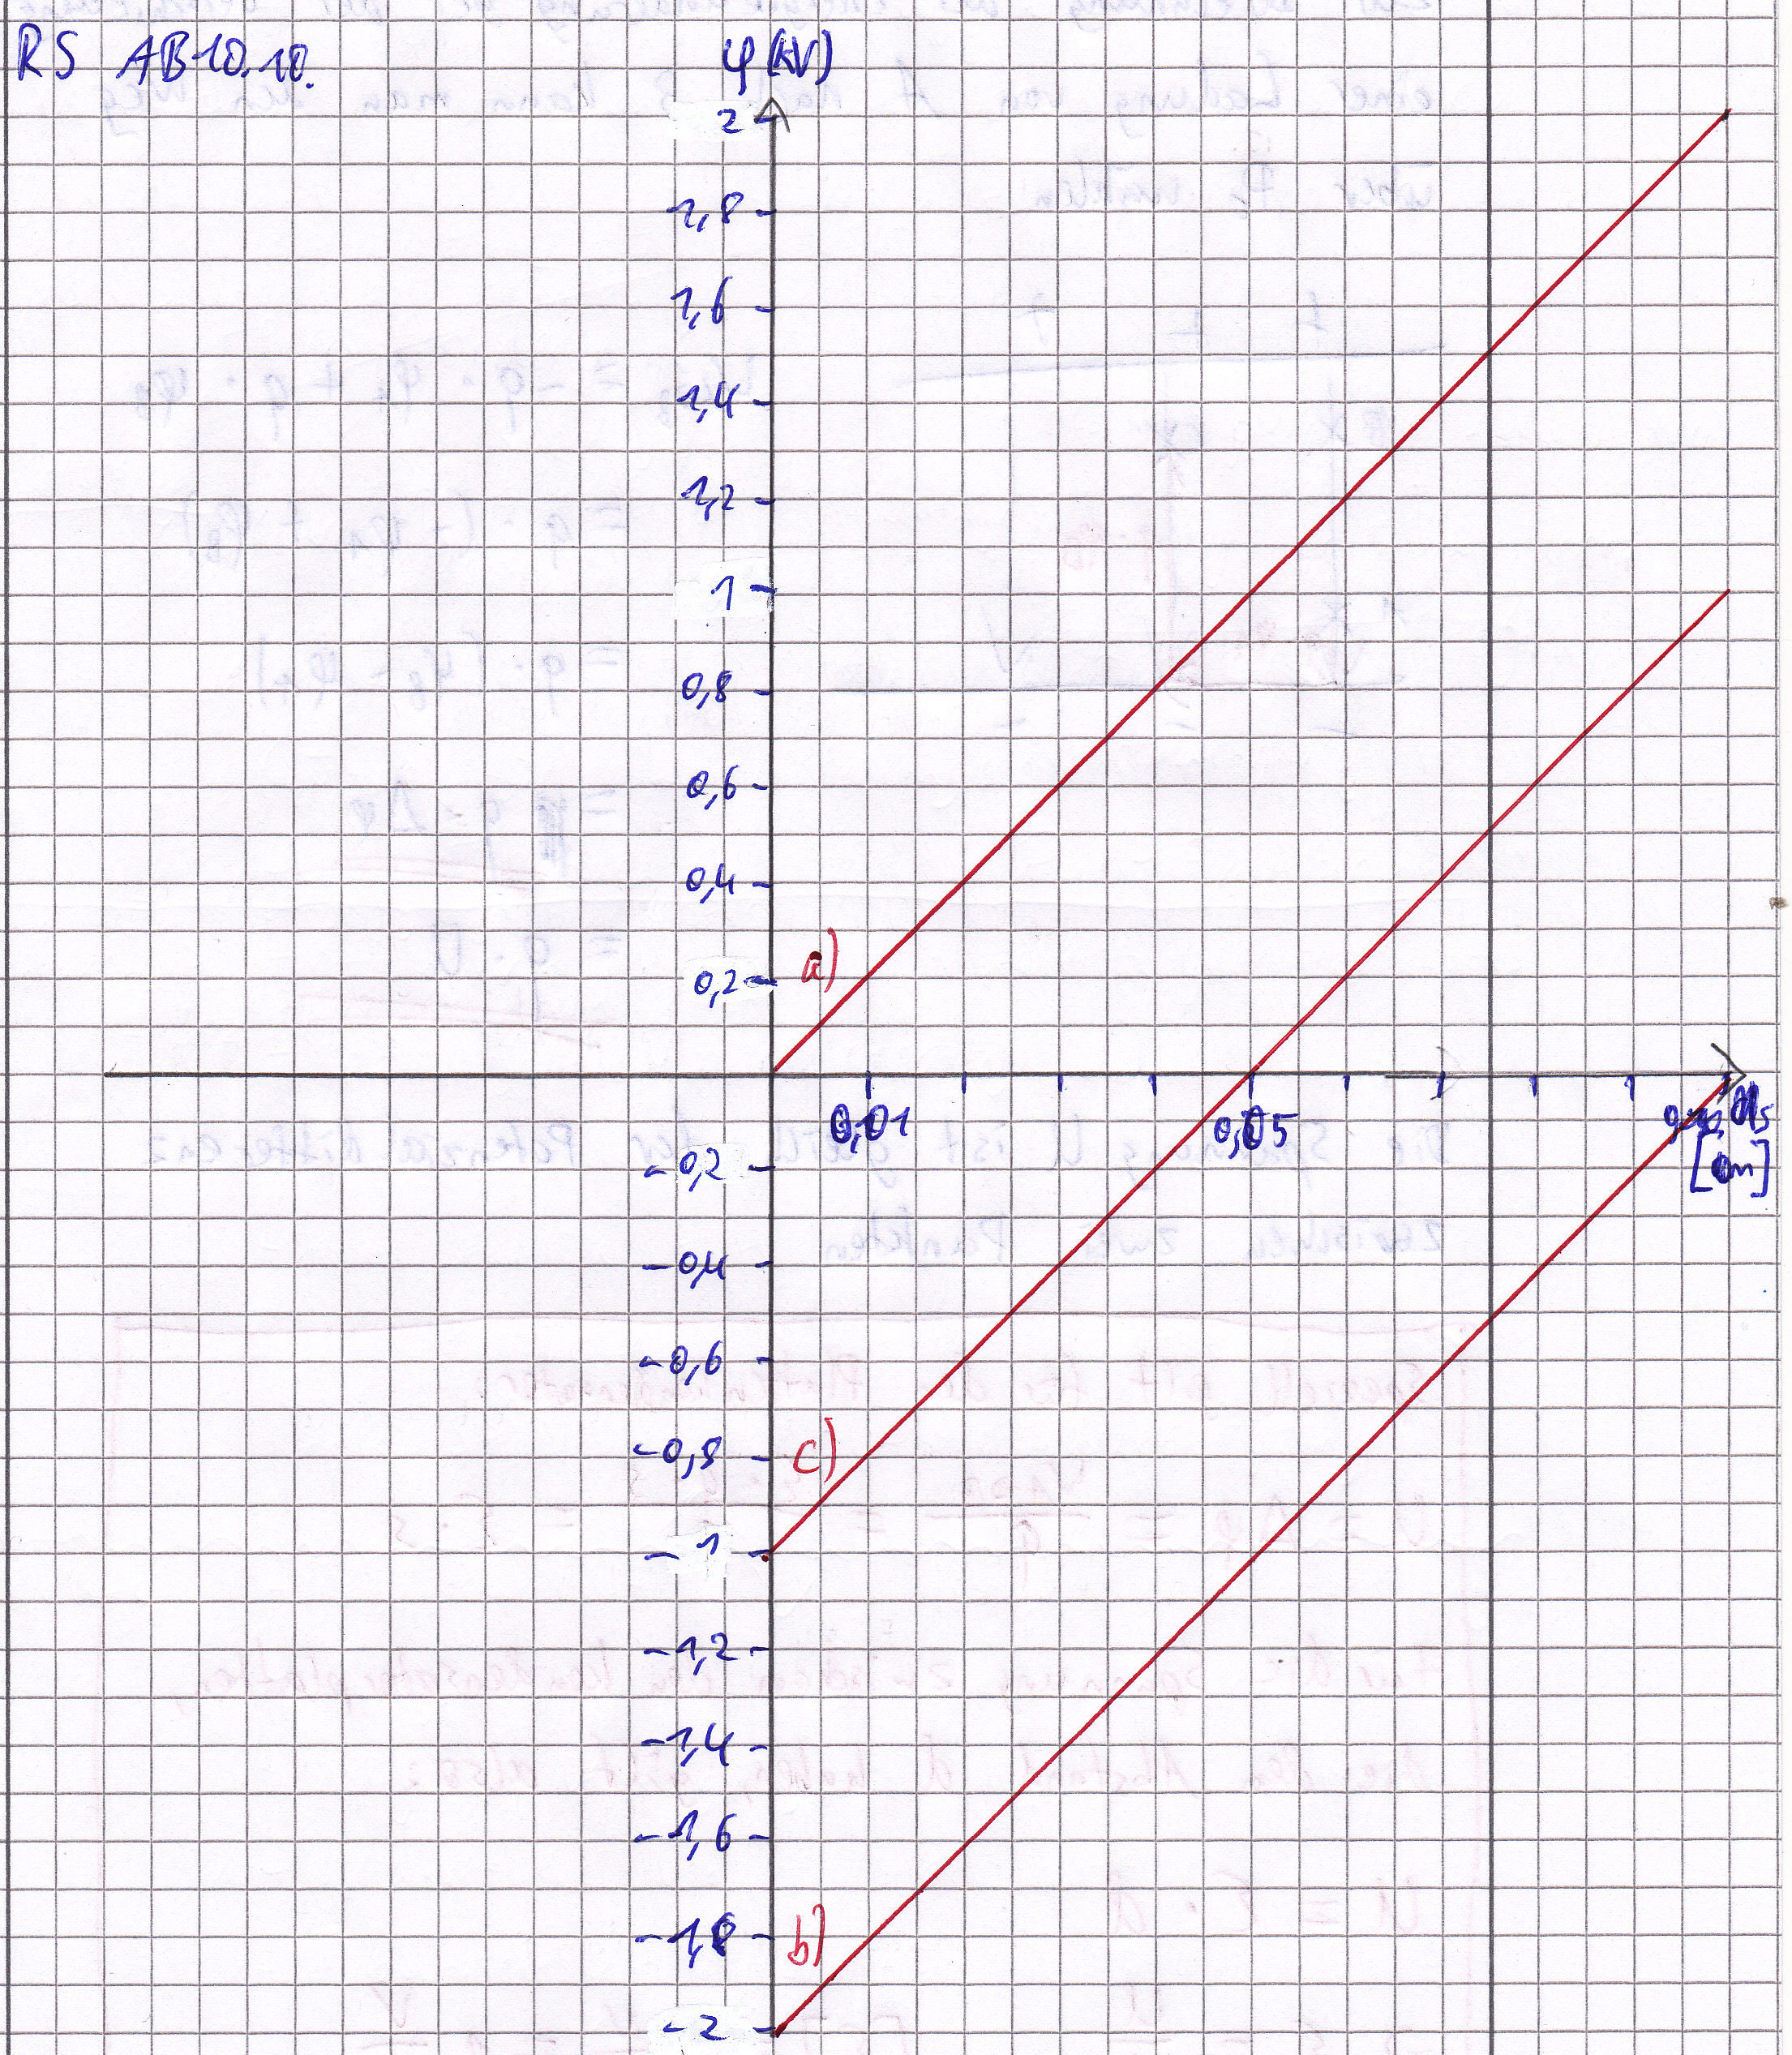
\includegraphics[scale=0.7]{I9_potential}
\vspace{2mm} \\
$\varphi_{(x)} = E \ast x + \varphi_{0}$ 

\vspace{2mm}
Bezugspunkte auf: \\
a) negativ geladener Platte \\
b) positiv geladener Platte \\
c) genau in der Mitte zwischen beiden Platten \\

\newpage

\subsubsection{Elektrische Spannung U}
Zur Berechnung der Energieänderung bei der Verschiebung einer Ladung von A nach B kann man den Weg über $P_{0}$ wählen. 

\vspace{2mm}
$ W_{A \rightarrow B} = -q \ast \varphi_{A} + q \ast \varphi_{B} $ \\
\hspace{11.5mm} $ = q \ast (- \varphi_{A} + \varphi_{B}) $ \\
\hspace{11.5mm} $ = q \ast \Delta \varphi $ \\
\hspace{11.5mm} $ = q \ast U  $ 
\vspace{2mm} \\
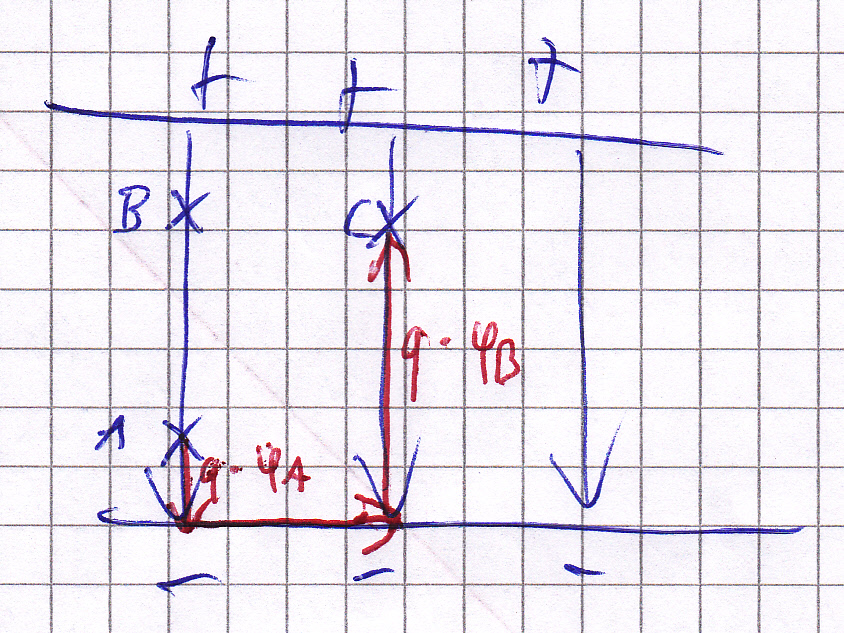
\includegraphics[scale=0.8]{I9_spannung}
\vspace{2mm} \\
Die Spannung U ist gleich der Potentialdifferenz zwischen zwei Punkten.

\vspace{5mm}
\underline{Speziell gilt für den Plattenkondensator:} \\
\vspace{2mm}
$ U = \Delta  \varphi = \dfrac{W_{A \rightarrow B}}{q} = \dfrac{E \ast q \ast s}{q} = E \ast s $

\vspace{2mm}
Für die Spannung zwischen den Kondensatorplatten, die den Abstand d haben, gilt also: \\
\vspace{2mm}
$ U = E \ast d $ \hspace{10mm} $ [E] = \dfrac{N}{C} = \dfrac{V}{m} $
\newpage
\subsubsection{Äquipotentiallinien}
Auf einer Fläche senkrecht zu den Feldlinien herrscht überall das gleiche Potential, da bei einer Verschiebung senkrecht zu den Feldlinien keine Energieänderung stattfindet. $\Rightarrow$ Äquipotentiallinien (unten in blau) \\
\vspace{3mm}
Je dichter die Äquipotentiallinien, desto größer die Energieänderung bei der Bewegung senkrecht dazu \\ $\Rightarrow$ desto größer ist die Feldstärke
\vspace{2mm}

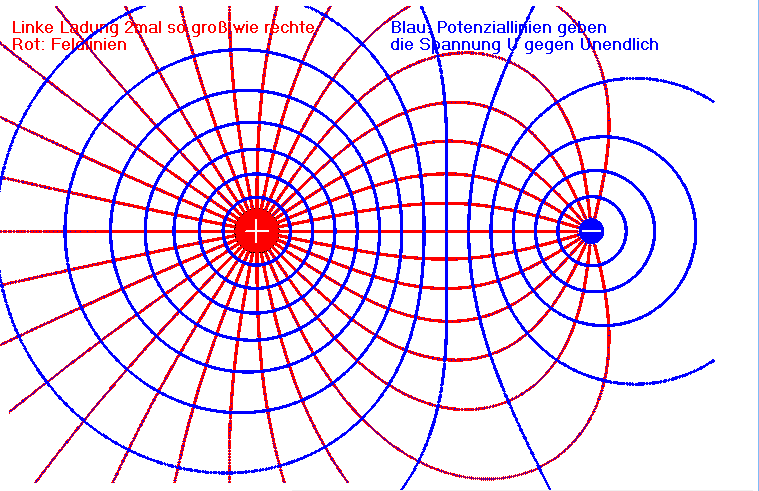
\includegraphics[scale=0.4]{I9_aequipotentiallinien}
\vspace{10mm}

\subsection{Geladene Teilchen im Längsfeld}
$ W_{A \rightarrow B} = q \ast U = q \ast \Delta \varphi $

\vspace{2mm}
Beim Durchfliegen der Beschleunigungsspannung U gewinnt das geladene Teilchen die Energie $ W = q \ast U $, falls die Spannung das Teilchen beschleunigt, andernfalls verliert dieses Energie (Siehe Buch S.20 B2).
\vspace{2mm} \\
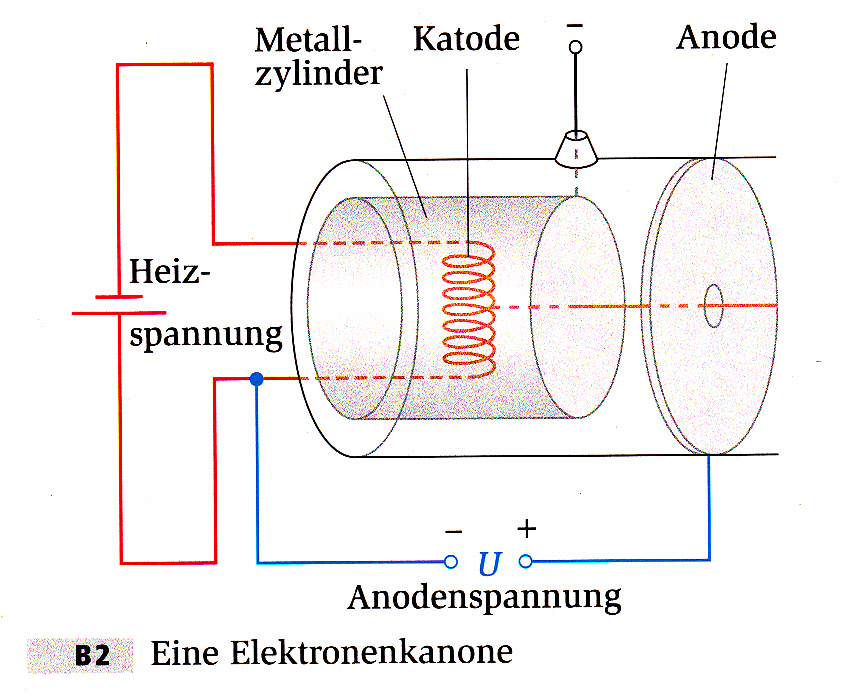
\includegraphics{I10_wehnelt}
\vspace{2mm} \\
Wird ein Elektron mit 250V beschleunigt, so hat dieses danach die Energiemenge $ W = q \ast U = e \ast U = e \ast 250V = 250 eV $ dazugewonnen.


\subsection{Kondensator-Kapazität}
\subsubsection{Ladung}
Wie viel Ladung fasst ein Kondensator bei vorgegebener angelegter Spannung U? (Bsp.: Plattenkondensator)
\vspace{2mm} \\
$ U = E \ast d $
\vspace{2mm} \\
Wir wissen bereits:
\vspace{2mm} \\
$ \sigma = \dfrac{Q}{A} $ und $ \sigma = \epsilon_{0} \ast E $
\vspace{2mm} \\
Daraus folgt:
\vspace{2mm} \\
\hspace{5mm}$ \dfrac{Q}{A} = \epsilon_{0} \ast E $\\ \vspace{4mm}$ \Rightarrow \dfrac{Q}{A} = \epsilon_{0} \ast \dfrac{U}{d} $\\ \vspace{4mm}$ \Rightarrow Q = \underbrace{\epsilon_{0} \ast \dfrac{A}{D}} \ast U $ \\
Konstante, genannt Kapazität C	

\vspace{5mm}
\underline{Allgemein gilt:}
Den Quotienten $\dfrac{Q}{U}$ nennt man Kapazität C. Die Ladung auf einem \\ \vspace{2mm}
Kondensator ist der angelegten Spannung proportional.

\vspace{5mm}
\underline{Merke:}
Anordnungen aus zwei Leitern, die durch einen Isolator getrennt sind, heißen Kondensatoren. Aufgrund ihrer Fähigkeit, Ladungen und Energie zu speichern, werden sie vielfältig eingesetzt. Die Kapazität C gibt an, wie viel Ladung der Kondensator bei einer bestimmten Spannung speichern kann:
\vspace{2mm} \\
$ C = \dfrac{Q}{U} $ \hspace{5mm} $ [C] = \dfrac{1C}{1V} = 1F $ (Farad; Nach Michael Faraday)
\vspace{5mm} \\
Symbol: 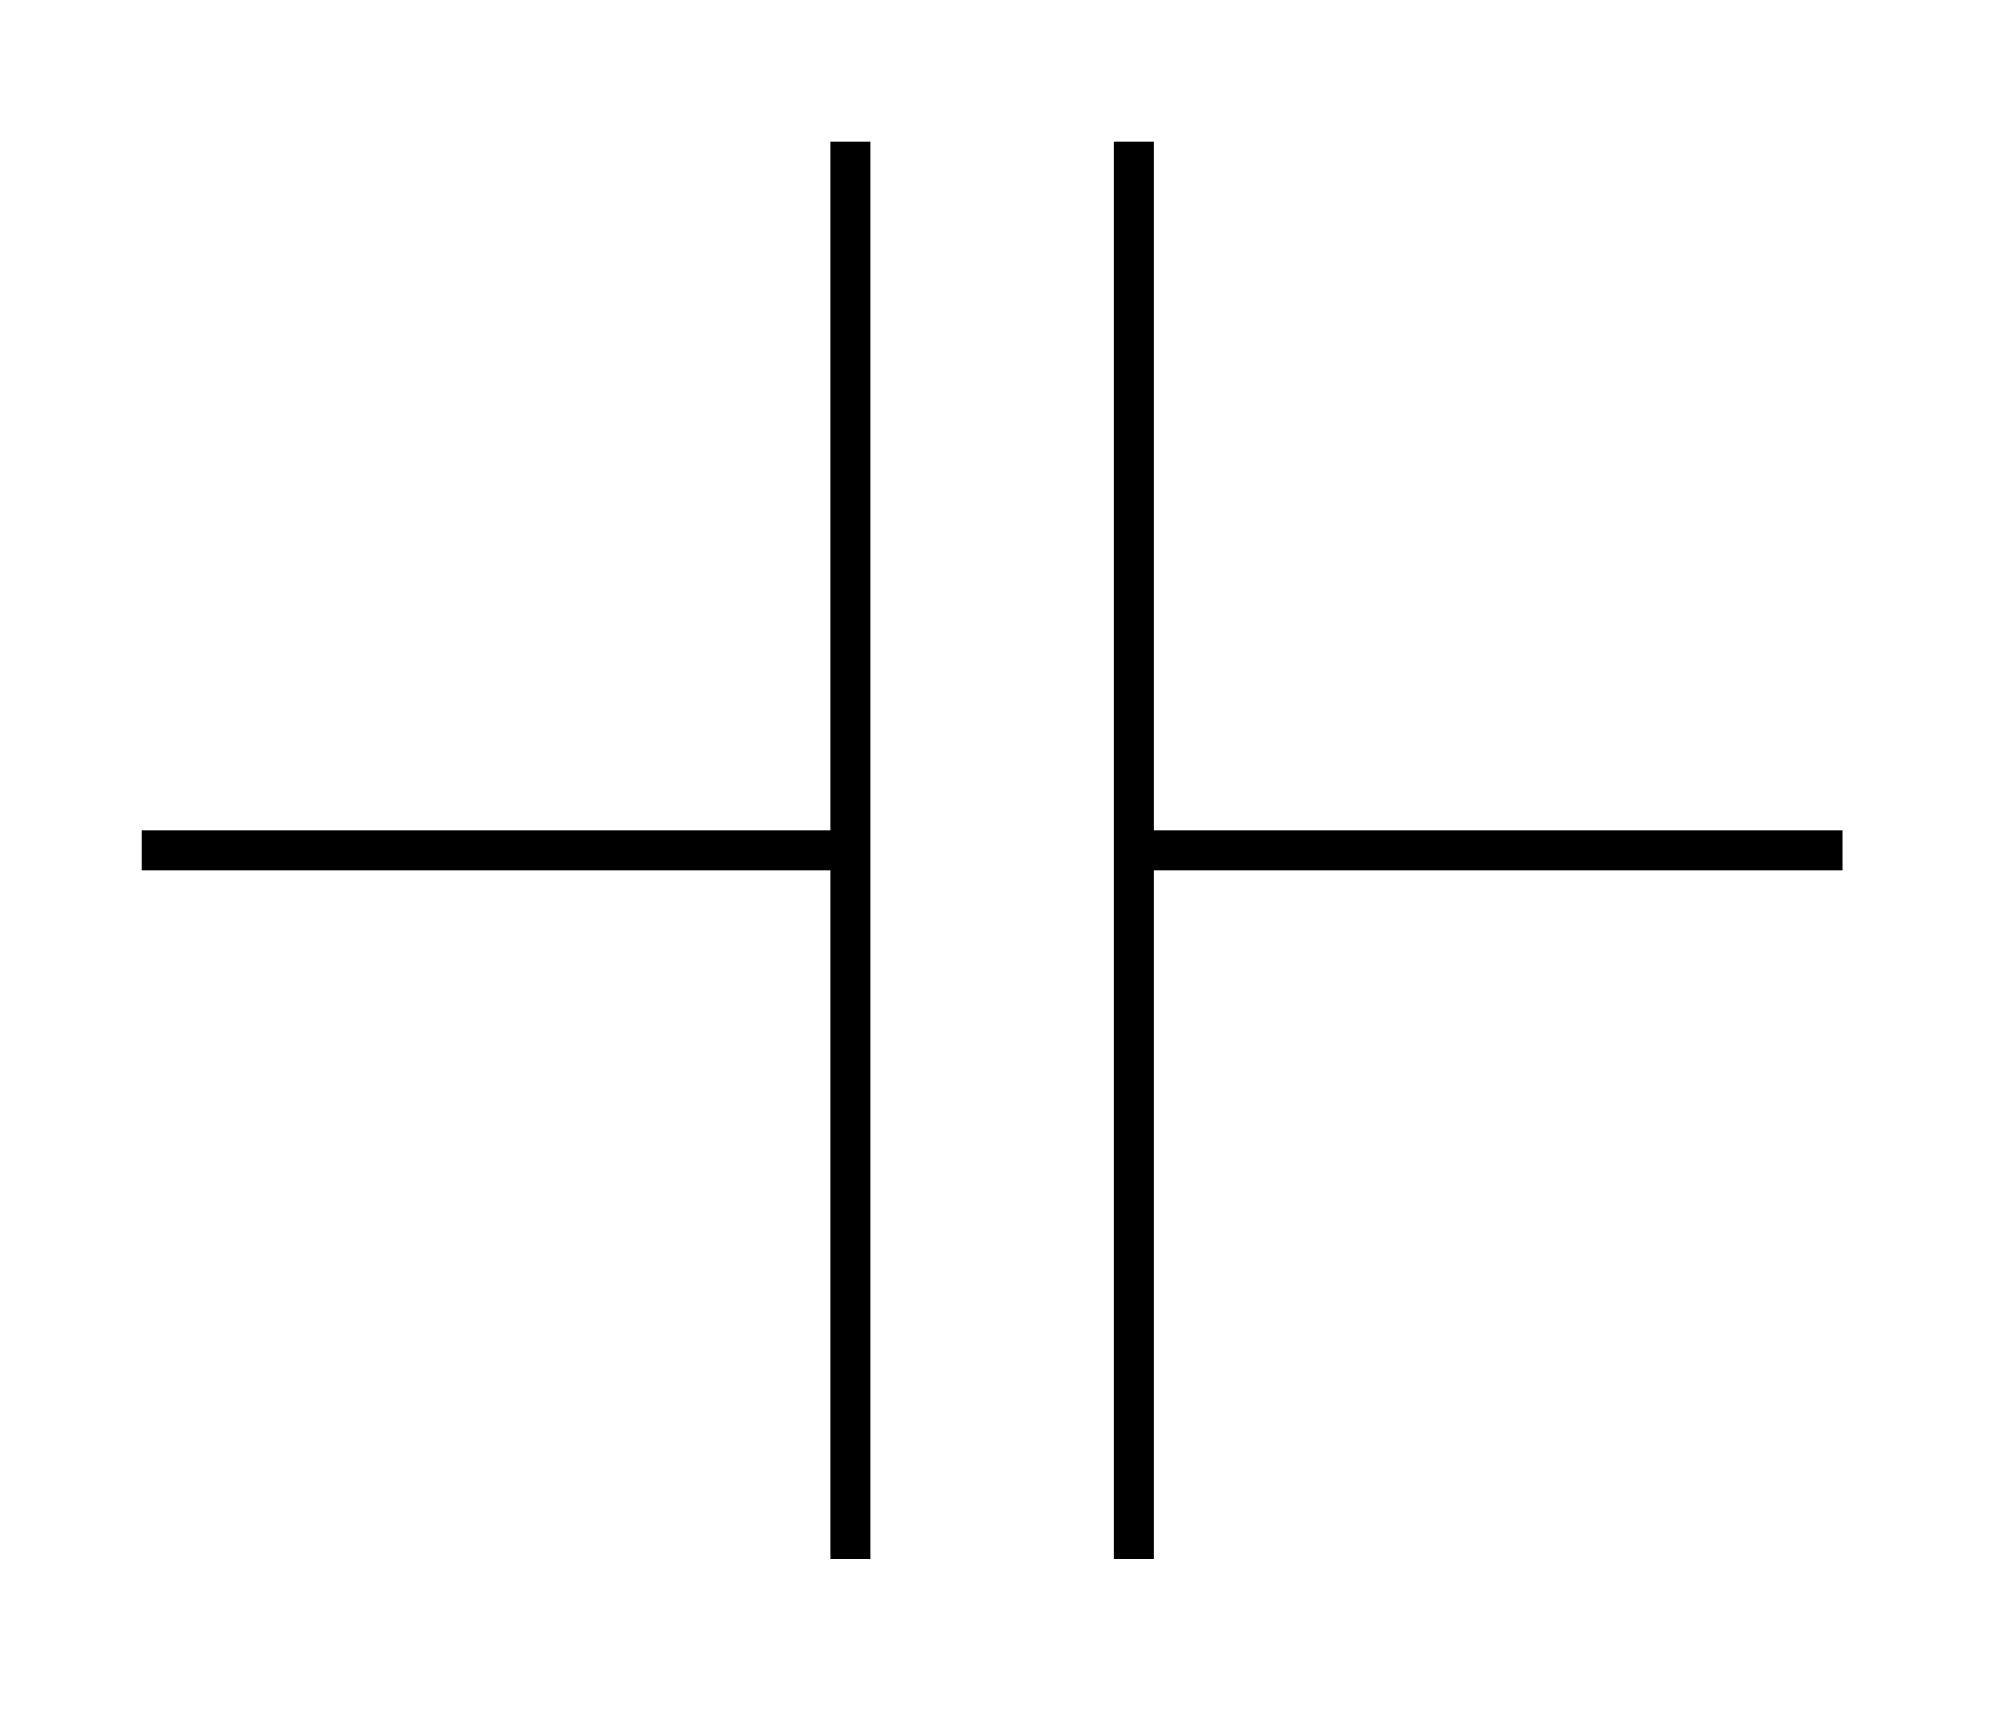
\includegraphics[scale=0.015]{capacitor}
\vspace{5mm} \\
Speziell: Die Kapazität eines \underline{Plattenkondensators im Vakuum} wird durch die Plattenfäche A und den Abstand D bestimmt. 
\vspace{2mm} \\
$ C = \epsilon_{0} \ast \dfrac{A}{d} $
\newpage
\subsection{Kondensator-Entladung und -Aufladung}
\underline{Schaltplan:}
\vspace{2mm} \\
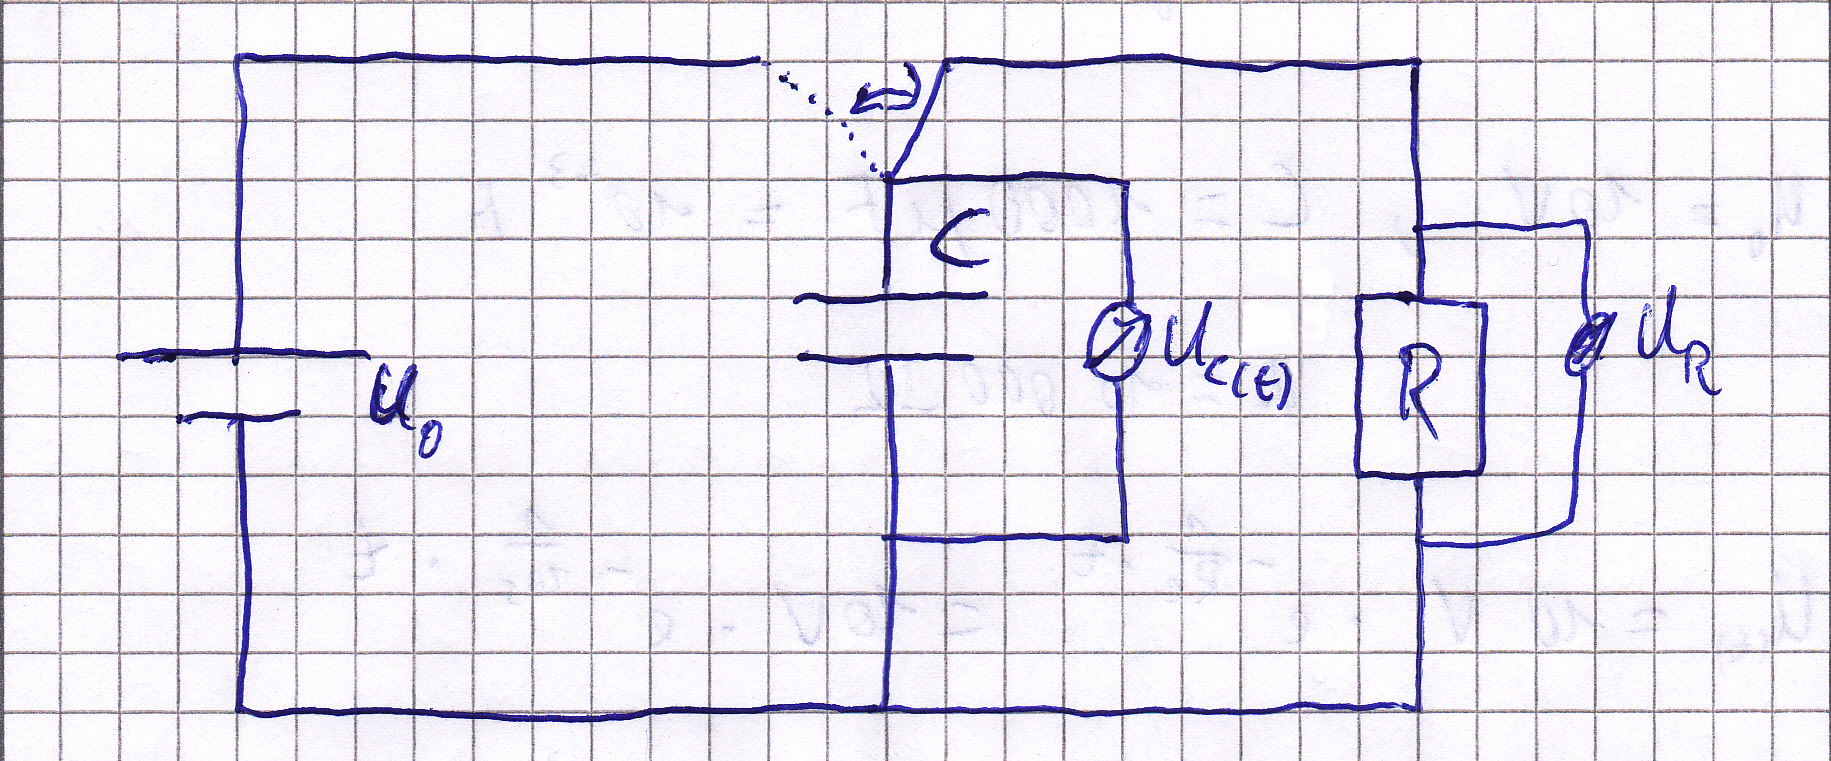
\includegraphics[scale=0.5]{I12_schaltplan}
\vspace{2mm}

$ U_{C(t)} = \dfrac{Q_{(t)}}{C} $
\vspace{2mm} \\
Bei uns: R = 10 k$\Omega$; C = 1000 $ \mu F $; $U_{0} = 10V$ \\
Beim Entladevorgang gilt: \\
\vspace{3mm}
$ U_{C(t)} = -R \ast I $ \hspace{40mm} (Maschenregel: $U_{C(t)} + U_{R} = 0$)
\vspace{5mm} \\
$ \dfrac{Q_{(t)}}{C} = -R \ast I $ \hspace{40mm} ( $\lim\limits_{\Delta t \rightarrow \infty}{\dfrac{\Delta Q}{\Delta t}} = \dot{Q}_{(t)}$ )
\vspace{5mm} \\
$ \dfrac{Q_{(t)}}{C} = -R \ast \dot{Q}_{(t)} $
\vspace{5mm} \\
$ \dot{Q}_{(t)} = \dfrac{Q_{(t)}}{\frac{C}{-R}} = \underbrace{\dfrac{-1}{C \ast R}} \ast Q_{(t)}$ \\
\hspace{24mm} Faktor
\vspace{5mm} \\
$ e^{x} = \dfrac{1}{0!}x^{0} + \dfrac{1}{1!}x^{1} + \dfrac{1}{2!}x^{2} + ... + \dfrac{1}{n!}x^{n}$ \hspace{2mm} $ \Rightarrow (e^{x})' = e^{x} $
\vspace{3mm} \\
\underline{Lösung:} $ Q_{(t)} = Q_{0} \ast e $ \hspace{15mm} $ \dot{Q}_{(t)} = Q_{0} \ast (-\dfrac{1}{C \ast R}) \ast e^{-\frac{1}{C \ast R} \ast t} $
\vspace{10mm} \\
$ U_{(t)} = \dfrac{Q_{(t)}}{C} = \underbrace{\dfrac{Q_{0}}{C}} \ast e^{-\frac{1}{C \ast R} \ast t} $ \\
\hspace{25.5mm} $U_{0}$
\vspace{5mm} \\
$ \dot{U}_{(t)} = - \dfrac{1}{C \ast R} \ast U_{(t)} $
\vspace{5mm} \\
$ 1F = \dfrac{1C}{1V} = \dfrac{1C}{1A \ast 1 \Omega} = \dfrac{1 As}{1A \ast 1 \Omega} = \dfrac{1s}{1 \Omega} $
\vspace{5mm} \\
$ F \ast \Omega = \dfrac{s}{\Omega} \ast \Omega = s $

\subsection{Mehrkapazität durch Isolatoren}
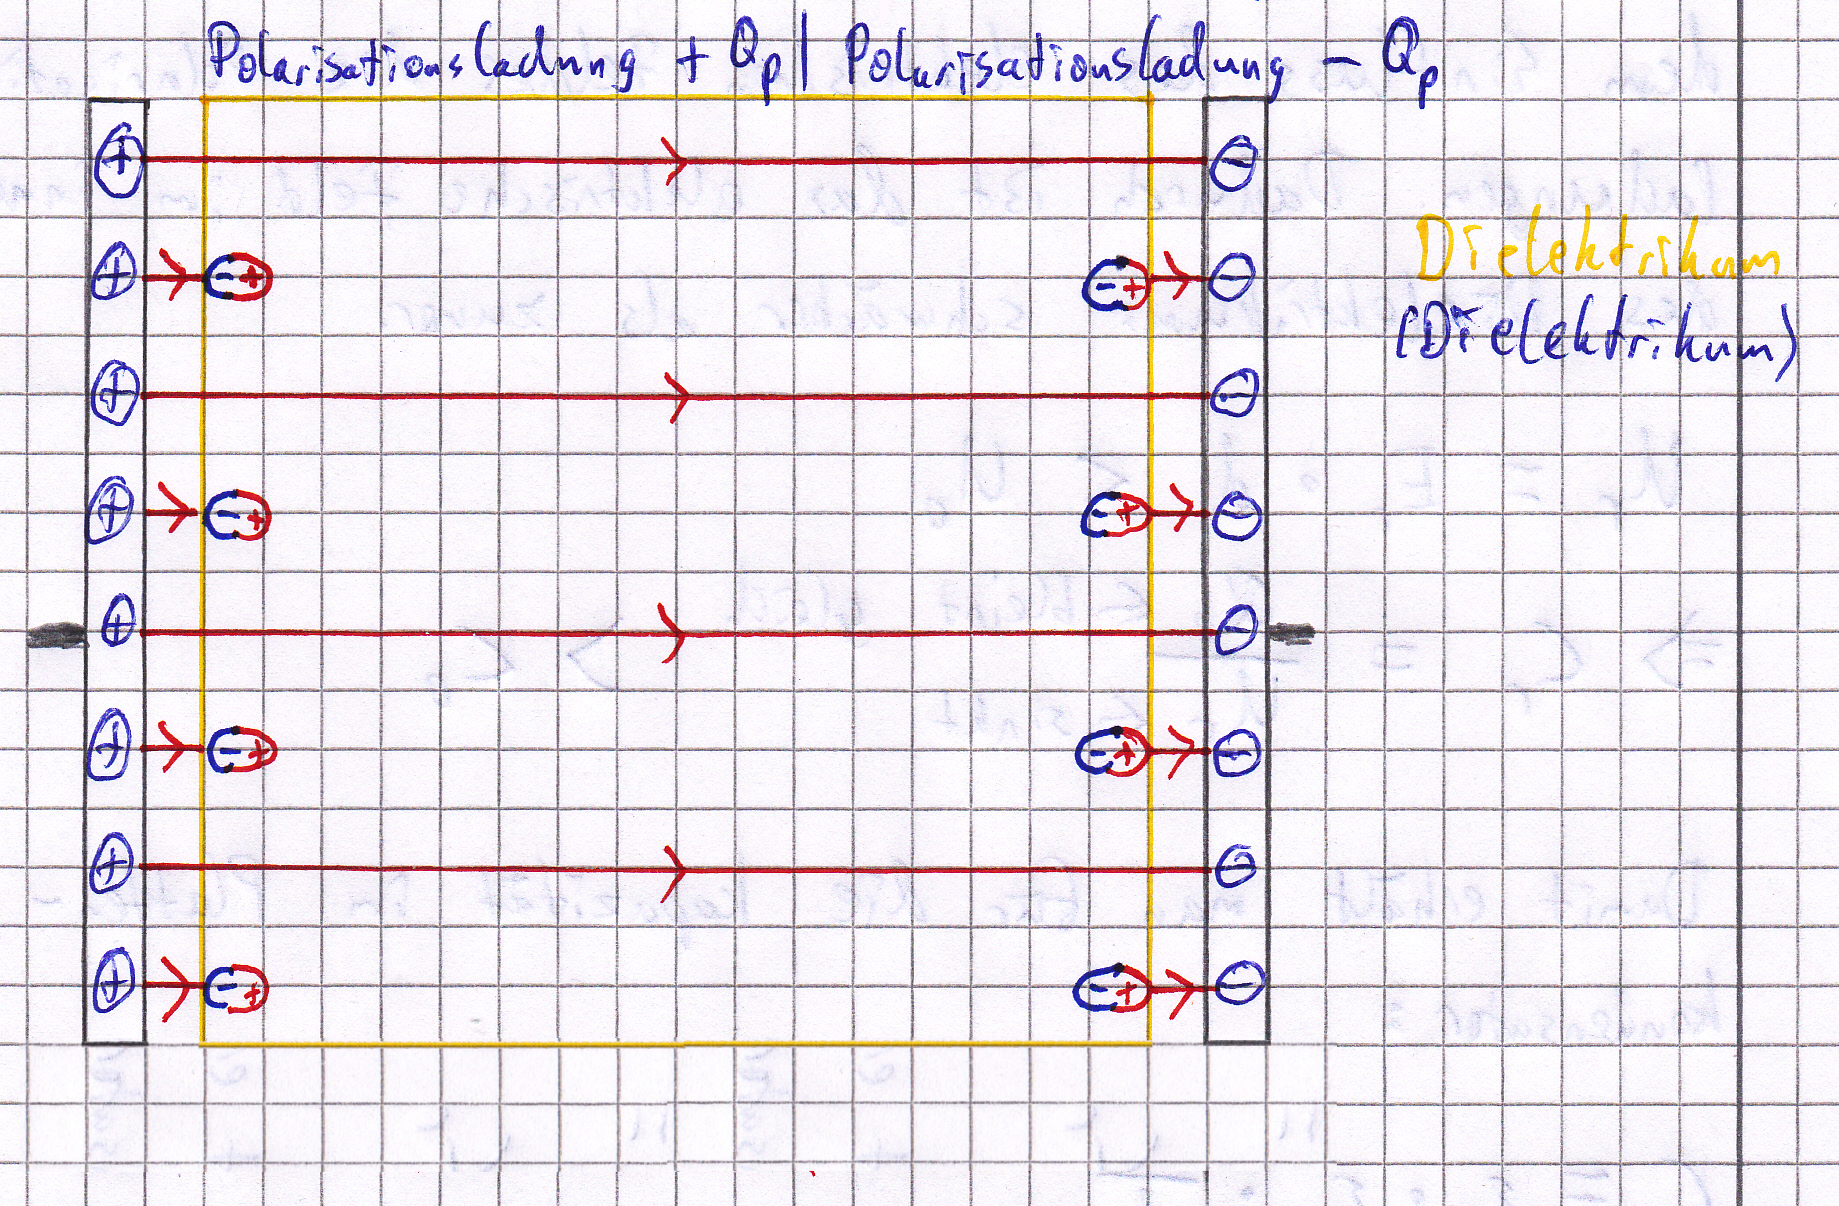
\includegraphics[scale=0.8]{I13_isolator} \\
\vspace{2mm}
$ E_{r} = \dfrac{E_{0}}{2} $ \hspace{20mm} (U = $ E \ast d $) 
\vspace{4mm} \\
$ \rightarrow U_{r} = \dfrac{U_{0}}{2} $
\vspace{4mm} \\
$ \rightarrow C_{r} = \dfrac{Q_{0}}{\frac{U_{0}}{2}} = 2 \ast C_{0} $
\vspace{6mm} \\
im Beispiel: $ \underbrace{\epsilon_{r}} = 2 $ \\
\hspace{12mm} Sprich: Epsilon r
\vspace{5mm} \\
\underline{Merke:} \\
In dem Isolator (Dielektrikum) verschieben sich unter dem Einfluss des elektrischen Feldes die Polarisationsladungen. Dadurch ist das elektrische Feld im inneren des Dielektrikums schwächer als zuvor. 
\vspace{5mm} \\
$ U_{r} = E_{r} \ast d < U_{0} $
\vspace{5mm} \\
$ \Rightarrow C_{r} = \dfrac{Q_{0} (\leftarrow bleibt)}{U_{r} (\leftarrow sinkt)} > C_{0} $
\vspace{3mm} \\
Damit erhält man für die Kapazität im Plattenkondensator: 
\vspace{2mm} \\
$ C = \epsilon_{0} \ast \underbrace{\epsilon_{r}} \ast \dfrac{A}{d} $ \\
\vspace{1mm}
\hspace{4mm} Dielektrizitätszahl

\subsection{Energie in elektrischen Feldern}
Wird der Kondensator aufgeladen, so steigt mit zunehmender Ladung Q auf den Kondensatorplatten auch die Spannung U. Um den Kondensator mit der zusätzlichen Ladung $\Delta Q$ weiter aufzuladen, ist die Energiemenge $\Delta W = \Delta Q \ast U_{(Q)} $ notwendig.
\vspace{2mm} \\
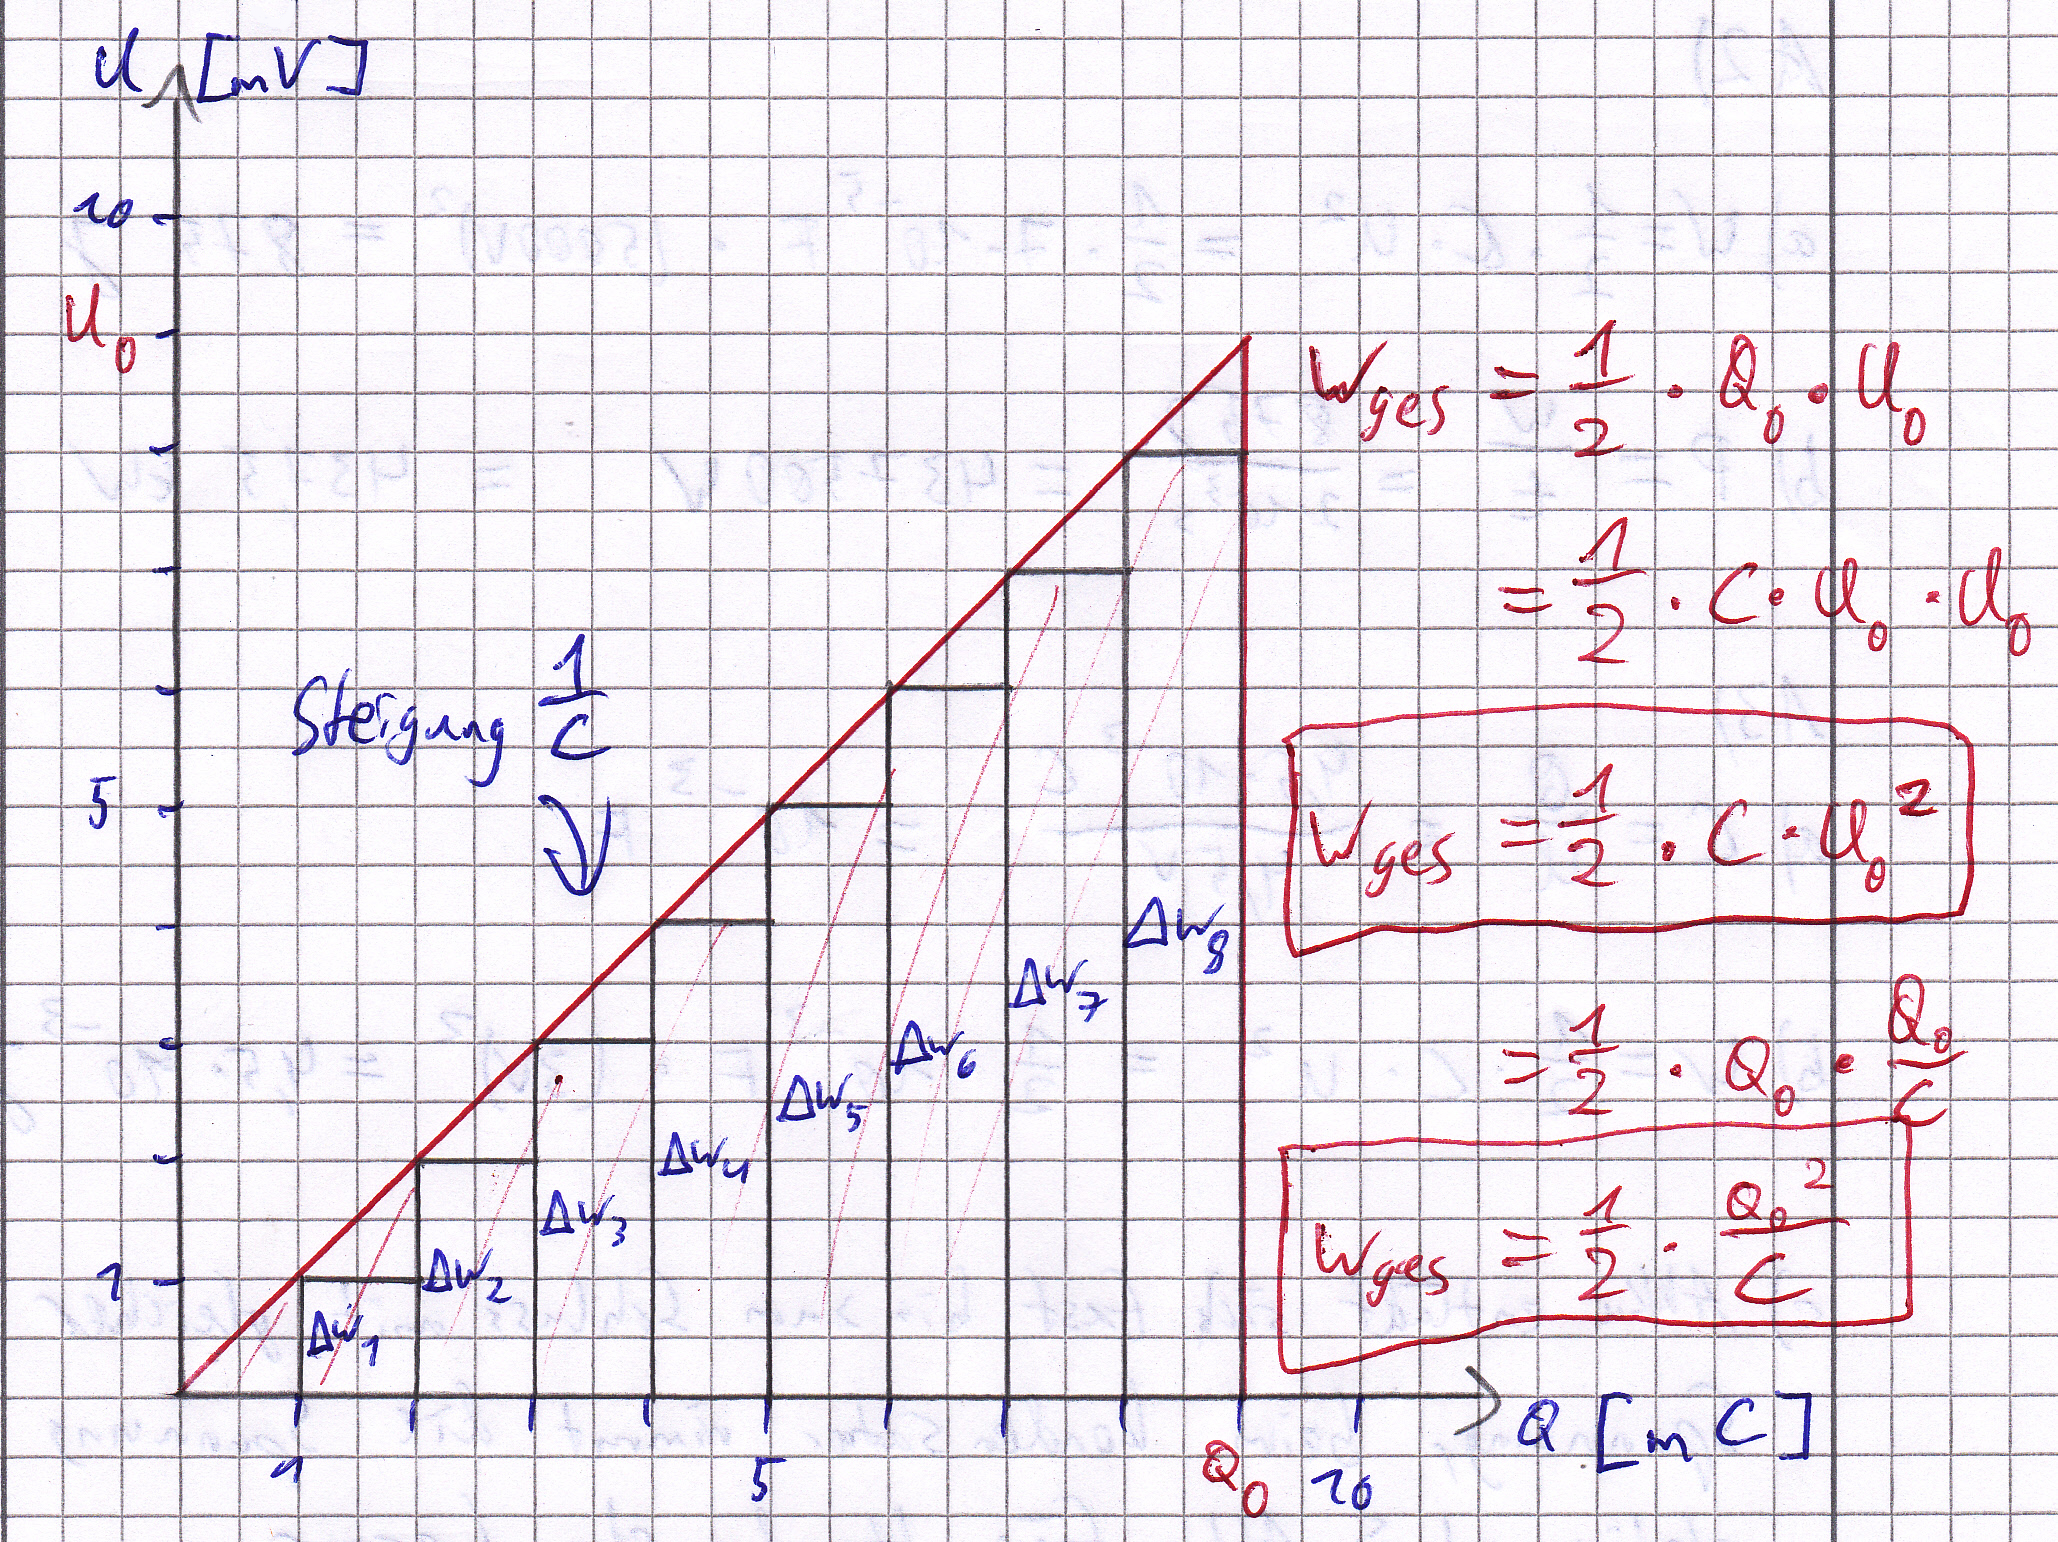
\includegraphics[scale=0.6]{I14_energie}
\vspace{2mm} \\
Die gesamte im Kondensator gespeicherte Energie ergibt sich aus dem Flächeninhalt unter dem Graphen im Q-U-Diagramm (Dabei ist $Q_{0}$ die Ladung, die der Kondensator am Ende trägt und $U_{0}$ die Spannung, auf die er aufgeladen wird).

\subsection{Parallel- und Reihenschaltung von Kondensatoren}
\subsubsection{Parallelschaltung}
$U_{ges} = U_{1} = U_{2}$
\vspace{2mm} \\
$Q_{ges} = Q_{1} + Q_{2}$
\vspace{2mm} \\
$C_{ges} = C_{1} + C_{2}$

\subsubsection{Reihenschaltung} 
$U_{ges} = U_{1} + U_{2}$
\vspace{2mm} \\
$Q_{ges} = Q_{1} = Q_{2}$
\vspace{3mm} \\
$\dfrac{C_{1}}{C_{2}} = \dfrac{U_{2}}{U_{1}}$
\vspace{3mm} \\
$\dfrac{1}{C_{ges}} = \dfrac{1}{C_{1}} + \dfrac{1}{C_{2}}$